\documentclass[11pt]{article}
\usepackage[english]{babel}
\usepackage[numbers]{natbib} 
\usepackage{url}
\usepackage[utf8]{inputenc}
\usepackage{amsmath}
\usepackage{amssymb}
\usepackage{graphicx}
\usepackage{parskip}
\usepackage{fancyhdr}
\usepackage{vmargin}
\usepackage{booktabs}
\usepackage[table,xcdraw]{xcolor}
\usepackage{tabularx}
\usepackage{caption} 
\usepackage{float}
\usepackage{longtable}
\usepackage{array}
\usepackage{caption}
\usepackage{subcaption}

\usepackage[colorlinks = true,
linkcolor = black,
urlcolor  = black,
citecolor = black,
anchorcolor = black]{hyperref}

\setmarginsrb{3 cm}{1 cm}{3 cm}{1 cm}{1 cm}{1.5 cm}{1 cm}{1.5 cm}

\newcolumntype{L}[1]{>{\raggedright\let\newline\\\arraybackslash\hspace{0pt}}m{#1}}
\newcolumntype{C}[1]{>{\centering\let\newline\\\arraybackslash\hspace{0pt}}m{#1}}
\newcolumntype{R}[1]{>{\raggedleft\let\newline\\\arraybackslash\hspace{0pt}}m{#1}}

\title{Assignment \#3 - Protein Classification}
\date{\today}

\makeatletter
\let\thetitle\@title
\let\thesubtitle\@subtitle
\let\theauthor\@author
\let\thedate\@date
\makeatother

\pagestyle{plain}

\captionsetup[table]{skip=5pt}

\makeatletter
\renewcommand*\l@section{\@dottedtocline{1}{1.5em}{2.3em}}
\makeatother


\begin{document}
	
%%%%%%%%%%%%%%%%%%%%%%%%%%%%%%%%%%%%%%%%%%%%%%%%%%%%%%%%%%%%%%%%%%%%%%%%%%%%%%%%%%%%%%%%%

\begin{titlepage}
	\centering
	\textsc{\LARGE University of Coimbra}\\[1.0 cm]
	\textsc{\large Doctoral Program in Information Science and Technology}\\[0.5 cm]
	\textsc{\large Real Time Learning in Intelligent Systems}\\[5 cm]
	\rule{\linewidth}{0.2 mm} \\[0.4 cm]
	{ \LARGE \bfseries \thetitle}\\ [0.2 cm]
	\rule{\linewidth}{0.2 mm} \\[3 cm]
	
	\textsc{Joaquim Pedro Bento Gonçalves Pratas Leitão - 2011150072}\\[5 cm]
	
	{\large \thedate}\\[2 cm]
	
	\vfill
	
\end{titlepage}

\tableofcontents

\newpage

%%%%%%%%%%%%%%%%%%%%%%%%%%%%%%%%%%%%%%%%%%%%%%%%%%%%%%%%%%%%%%%%%%%%%%%%%%%%%%%%%%%%%%%%%

\section{Introduction}
\label{introduction}

The protein classification problem is among the most important and fundamental problems in computational biology. In short, this problem can be defined as the task of classifying proteins into functional and structural classes based on \emph{homology} (evolutionary similarity) of protein sequence data.

Several approaches can be taken to solve the protein classification problem, ranging from methods that analyse the protein's coding sequence in the genetic code, to more complex approaches that study the 3D structure of the proteins in order to perform such classification.

In the current assignment, a sequence similarity-based approach to this problem will be adopted. The algorithms and methods to be applied fall in the first set of practices mentioned in the previous paragraph. As such, the current work will focus on analysing the genetic sequence responsible for coding a given protein. Browsing solutions for this problem proposed in the literature Support Vector Machines appear as interesting techniques, achieving promising results \cite{leslie2002mismatch, zavaljevski2002support, cai2003svm}.

\subsection{Objectives}

One major high-level objective can be identified in the present assignment: For any given protein determine its functional class by analysing its coding sequence.

This work will feature data from the \emph{SCOP Database}\cite{murzin1995scop}, more precisely the \emph{SCOP40} dataset\footnote{\url{http://pongor.itk.ppke.hu/benchmark}}. This dataset contains genetic sequences responsible for coding proteins of 55 different families. Therefore, a more low-level objective for this work is to develop classifiers capable of identifying protein sequences belonging in each of the 55 families.

The current assignment also featured a secondary objective, consisting in comparing incremental with non-incremental classifier approaches. 

\subsection{Methodology}
\label{methodology}

In light of the description of the assignment at hand, and its objectives, the following steps will be considered in the work to be performed:

\begin{enumerate}
	\item Initial dataset preprocessing
	
	\item Data representation
	
	\item Classifier training
	
	\item Results assessment
\end{enumerate}

In an initial stage, a preprocessing of the \emph{SCOP40} data was conducted, aiming to construct a training and testing dataset for each one of the 55 families in the dataset. It is worth mentioning that even though the \emph{SCOP Database} does not provide separate training and testing datasets for each family, it proposes a list of instances to be used for training and testing, for each family. Therefore, at this stage, the preprocessing step consisted in analysing the provided mapping and in creating individual train and test files for each family.

Probably the most important step in this assignment, data representation can be seen as an advanced preprocessing step to transform the data to be feed to a classifier. It strongly conditions the final performance of the classifiers as an inappropriate representation does not allow for a good separation of the data, therefore leading to poor classification performance. In this work the \emph{segmentation} was the representation technique implemented. Section \ref{data_representation} covers this technique in detail.

Following the representation classifiers needed to be properly trained and tested. In this work \emph{incremental} and \emph{non-incremental} classifiers were intended to be compared. In this sense two different but somewhat related classifiers were selected: \emph{LASVM}, as the incremental classifier; and \emph{Support Vector Machines (SVM)}, as the non-incremental classifier.

As each protein sequence under analysis must be assigned to one of 55 possible families, a multi-class classification problem is being considered. In this sense one classifier for each family must be develop. Considering that two different classifiers are intended to be compared, two classifiers were trained for each family (one \emph{LASVM} and one \emph{SVM}).

Finally, once the classifiers were properly created and trained, their performance was assessed with the testing dataset, following an analysis of the test results in order to determine which approach registered better results, if any. Considering the fact that the \emph{SCOP40} is an highly unbalanced dataset (indeed, a fact that is very common in problems of this nature in computational biology) the different approaches were not compared with respect to their accuracy, but with respect to the \emph{Area Under Curve} metric.

Concerning the classifiers' development and all \emph{assignment-related} tasks, the \emph{R}\footnote{\url{https://www.r-project.org/}} software environment was selected as the implementation and working tool.

\subsection{Document Outline}

The remainder of this document is organised as follows: Section \ref{dataset_description} introduces and describes the dataset used in the current work. Section \ref{data_representation} addresses the data representation technique adopted in this assignment. Sections \ref{svm} and \ref{lasvm} cover the experimental results obtained with the two techniques being compared in this work. Finally, section \ref{conclusions} presents a reflective analysis of the obtained experimental results and identifies directions to be explored in future work.


\section{Dataset Description}
\label{dataset_description}

The \emph{SCOP40} dataset contains information concerning the genetic coding sequences of different proteins and their corresponding families, being organised in two main files, as follows:

\begin{itemize}
	\item \emph{SCOP40mini.fasta} - Text file listing the different genetic coding sequences for several proteins. A unique identifier is also presented for each protein sequence.
	
	\item \emph{SCOP40mini\_sequence\_minidatabase\_19.cast} - Text file containing a mapping between each family and the protein sequences of the \emph{SCOP40mini.fasta} file to be used during classifier training or test.
\end{itemize}

\section{Data Representation}
\label{data_representation}

Referenced in subsection \ref{methodology}, the representation technique implemented in the current work was the \emph{segmentation} method. In short, this method consists in, for each protein sequence, count the number of occurrences of each individual nucleotide (that is, of each letter in the sequence).

For example, consider the following example protein sequence: \emph{"vdaeavvqqkcis"}. The segmentation method would output a total number of 3 occurrences for the \emph{"v"} nucleotide, 1 occurrence for the \emph{"d"} nucleotide, and so on. The only exception is for \emph{"x"} nucleotides, which represent missing information about a nucleotide in the protein sequence, and therefore are discarded in this exercise. Figure \ref{representation_example} presents an example of the output of this method for a protein sequence. 

\begin{figure}[h]
	\centering
	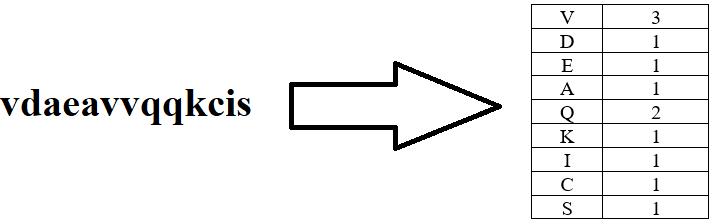
\includegraphics[scale=0.7]{images/representation.png}
	\caption{Example of the implemented segmentation representation for a protein sequence.}
	\label{representation_example}
\end{figure}

As it is not mandatory that each protein sequence contains all possible individual nucleotides, this method requires an initial passage for all the sequences in the dataset, in order to identify all individual nucleotides. The method's output will, therefore, present the number of occurrences of each of those nucleotides in the current protein sequence being analysed.

\section{Support Vector Machines}
\label{svm}

\emph{Support Vector Machines} (SVM) \cite{cortes1995support} are supervised machine learning algorithms applied in classification and regression tasks. During SVM training a model is built using a set of labelled samples (which can belong to one of two possible classes). Such model can then be used to classify new samples, that is, assign a new sample to a previously defined and learned class.

During training an hyperplane that assures the largest separation between instances of both classes is sought. The data points that lie closest to the hyperplane are called \emph{support vectors} and determine the separation margin between the two classes. Because of their (usually) small distance to the separation hyperplane these are the most difficult data points to classify. Misclassification of some instances may or may not be allowed. Such behaviour is controlled by a \emph{cost} parameter $C$ that penalises misclassification.

Even though SVMs seek a linear hyperplane, and therefore perform a linear classification task, they have also been extensively applied in non-linear classification problems. When performing non-linear classification, SVMs need to map the samples into a higher dimensional space, where a linear separation hyperplane can be computed. Once such a hyperplane has been determined an inverse transformation can be performed, mapping the data back to the original space. Such mapping operation is defined as a \emph{kernel}. For this reason, and since most \emph{application} problems are non-linear, SVMs are considered \emph{kernel methods}.

Several high-dimensional mappings, or \emph{kernels}, have been proposed in the literature for SVMs, though typical kernels covered in SVM books include: \emph{linear}, \emph{polynomial}, \emph{sigmoid} and \emph{radial basis function} (RBF).

In the current work, SVMs featuring a RBF kernel are intended to be applied. RBF kernels are defined by the following mathematical expression: $exp(- \gamma * |x_{i}-x_{j}|^2) $. Therefore, SVM training and classification performance will be influenced by the values defined for the cost and RBF parameters: $C$ and $\gamma$, respectively.

As no prior knowledge of adequate values for these parameters has been obtained, optimal values must be searched. As suggested by Hsu \emph{et al.} \cite{hsu2003practical}, a good practice to tune these parameters is to perform a grid search with exponentially growing sequences of $C$ and $\gamma$ (for example $C \: = \: 2^{-5}, 2^{-4}, \cdots , 2^{5}$ and $\gamma \: = \: 2^{-15}, 2^{-14}, \cdots , 2^{3}$).

As mentioned in \ref{methodology}, all algorithms used throughout the work were implemented in the \emph{R} software environment. With respect to SVMs, the \emph{e1071}\footnote{\url{https://CRAN.R-project.org/package=e1071}} package was used, providing an interface in the R programming language for the popular SVM library, \emph{LIBSVM} \cite{CC01a}.

\textbf{FIXME: Apresentar aqui os resultados! No fundo dizer quais foram as combinações de parâmetros que testámos e quais é que nos deram os melhores resultados para cada família; Apresentar valor médio de AUC das melhores abordagens nas 55 famílias}

\section{LASVM}
\label{lasvm}

\textbf{FIXME: Explicação teórica + referência biblioteca, etc}


\textbf{FIXME: Apresentar aqui os resultados! No fundo dizer quais foram as combinações de parâmetros que testámos e quais é que nos deram os melhores resultados para cada família}

\section{Conclusions}
\label{conclusions}

\bibliographystyle{unsrtnat}
\bibliography{bibliography}

\end{document}